\documentclass[a4paper,10pt]{article}
%
\usepackage{amsmath}
\usepackage{amssymb}
\usepackage{amstext}
\usepackage[bookmarks,colorlinks]{hyperref}
\usepackage{makeidx}
\usepackage{graphicx}
\usepackage{longtable}
\usepackage{multirow}
\usepackage{listings}
\usepackage{xcolor}

\makeindex

\usepackage{geometry}
\geometry{left=3cm,right=4cm,top=4cm,bottom=4cm}

\lstset{numbers=left, numberstyle=\tiny, basicstyle=\tiny, keywordstyle=\color{blue!70}, commentstyle=\color{red!50!green!50!blue!50}, frame=shadowbox, rulesepcolor=\color{red!20!green!20!blue!20},escapeinside=``, xleftmargin=2em,xrightmargin=2em, aboveskip=1em}

\begin{document}
%-----------------------------------------------------------

\title{Technical Report of MF optimization}
\author{Wei Cao}
\maketitle
%--------------------------------------------------
\begin{abstract}\
MF is \emph{Message Framwork} for short, this document introduces concepts and structure of MF briefly and then presents optimizations fulfilled by Wei Cao and Peisheng Wang.

Wei focuses on reducing the number of messages transferred between managers and minimize the synchronization cost within multiple threads.
\begin{itemize}
\item Wei improves the Direct Communication mode in MF to make Client generate unique request IDs itself and information of services that are frequently accessed is cached,
so that Client need not ask for permission from Controller each time it requests services.
\item A batch-request interface is also provided for Client to send a series of requests to Server with much less messages transferred.
Experiments shows, less messages between managers could shrink network IO overhead significantly.
\item Besides, Wei makes a lot of efforts in minimizing multiple threads' synchronization cost caused by locks and busy waiting(polling), in both MF-full and MF-light.
For example, queues, mutexs and semaphores are used to avoid busy waiting, to gain performance as much as possible, a fast and lightweight sempahore implementation is written to replace the one in boost.
Wei rewrites lot of code in MF-light to decrease scope of locks everywhere and remove needless locks.
\item Wei still tries other methods to optimize MF, for example, use multiple threads for serializing and deserializing messages and write a thread pool to manage these threads,
this method can increase throughput under heavy load.
\item Wei's optimization improves performance of both MF-full and MF-light.On testbed, in MF-full, indexing time is cut down by 82.9\%, while query time is cut down by 82\% to 91\% depending on query words.
While in MF-light, indexing time is cut down by 65\%, while query time is cut down by 56\% to 76\%.
\end{itemize}

Peisheng focuses on improving serialization efficiency.
\begin{itemize}
\item Original MF adopts boost ::serialization majorly for serialization, however, boost is not as fast as other serialization methods, such as febird and memcpy.
Peisheng implements a hierarchical serialization framework, it's a flexible and scable framework and can support all the three kinds of serialization methods mentioned above.
\item Besides, Peisheng uses MFBuffer instead of VariantType, saving both compile time and runtime efficiency,
and merges three similar classes ServiceRequestInfo ,ServiceResult, and ServiceMessage together to be one single class to avoid 
runtime conversion and also make batch request more efficient.
\item Peisheng also supplies a new type of batch-request interface, application layer batch-request, which is much flexible. To make MF easier to use, Peisheng provides some macros for MF user.
\item Experiments shows, on testbed, query is 20\% faster than before, the amount of data tranferred over MF greatly, only 10.74\% percent compared with the old one, 
the performance gain comes from time cost on sending and receiving messages in MF, besides indexing are 50\% faster than before.
\end{itemize}

A rough observation of Sf1 with optimized MF shows, query is 300\% faster than before.
\end{abstract}

%--------------------------------------------------
\tableofcontents
%--------------------------------------------------

\section{Document History}
\begin{center}
\begin{tabular}{|c|c|p{7cm}|}
    \hline
    Date & Author & Description \\ \hline
    2009-07-12& Wei Cao & Create the technical report. \\ \hline
    2009-07-21& Peisheng Wang & Add serialization framework and related improvement on MF. \\ \hline
    2009-07-23& Wei Cao & Add abstract. \\ \hline
\end{tabular}
\end{center}

\section{Overview}
\subsection{Components in MF}
\index{Message Framework, MF}
Message Framework is a communication tools among the managers. In Message Framework, there are three logical components which are: \emph{MessageClient}, \emph{MessageServer}, and \emph{MessageController}.
\begin{enumerate}
 \item \emph{MessageClient}
 \index{MessageClient}

 MessageClient requests services of connected manager to the MessageController and gets the result from MessageController or from MessageServer.
 \item \emph{MessageServer}
 \index{MessageServer}

 MessageServer registers services, which MessageServer can serve, to the MessageController and serves the result of service request from MessageController or from MessageClient.
 \item \emph{MessageController}
 \index{MessageController}

 MessageController processes registration of the MessageServer and serves information of available services to the MessageClient. In other words, MessageController controls messages of MessageClient and MessageServer.
\end{enumerate}

\subsection{Communication Modes}

There are two ways to communicate each other: Normal Communication and Direct Communication, as show in Figure \ref{fig:mf_orig}.
\begin{enumerate}
\item{Normal Communication:}
\index{Normal Communication}

MessageClient requests service to the MessageController. MessageController determines where the request goes and delivers it to the right MessageServer.
MessageServer processes the request and gives the result of request to the MessageController. Then finally MessageController delivers the result to the MessageClient.
\item{Direct Communication:}
\index{Direct Communication}

MessageClient requests service the MessageController. MessageController lets both MessageClient and MessageServer know that it is the time to use Direct Communication.
After MessageServer processes the result of the service which is given by MessageClient, it serves the result to the MessageClient directly.
\end{enumerate}

\begin{figure}[!ht]\centering
  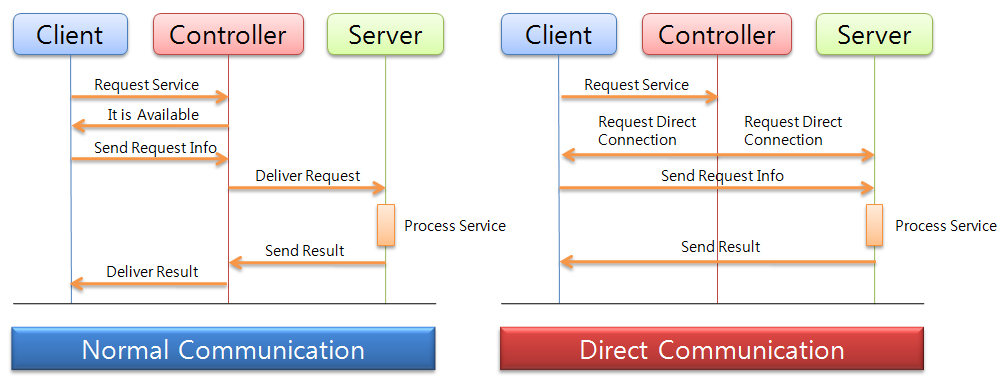
\includegraphics[width=1.00\textwidth]{mf_1.png}
  \caption{Two types of communication modes supported by MF}\label{fig:mf_orig}
\end{figure}

Direct Communication is faster and used more frequently than Normal Communication, so the following optimization focus on Direct Communication.

\subsection{MF-full and MF-light}

MF is designed to be highly flexible, managers can be binded to any number of processes and deployed to one or more machines arbitraily.
Usually managers are divided into serveral different processes, and MF-full is applied.
But sometimes, if the amount of computation is not so large, and all managers could be placed inside a single process, MF-light is designed to optimize such kind of usage.
\begin{enumerate}
\item{MF-full:}
\index{MF-full}

Because managers are distributed to different processes which may be deployed to different machines, MF-full is implemented through socket and messages are transferred via network.
\item{MF-light:}
\index{MF-light}

MF-light is much more lightweight and therefore faster than MF-full, MF components invoke each other directly, and messages are transferred by reading and writing shared queues.
\end{enumerate}
There is some macros in the head file message\_framework.h, you can modify them to select MF-full or MF-light at compile time.

\subsection{Hierarchical structure of MF-full}
\index{hierarchy}

Implementation of MF-full adopts a hierarchical structure, there are four layers in MF-full, Figure \ref{fig:mf-full} shows how data flow between layers when managers communicate with each other.

\begin{figure}[!ht]\centering
  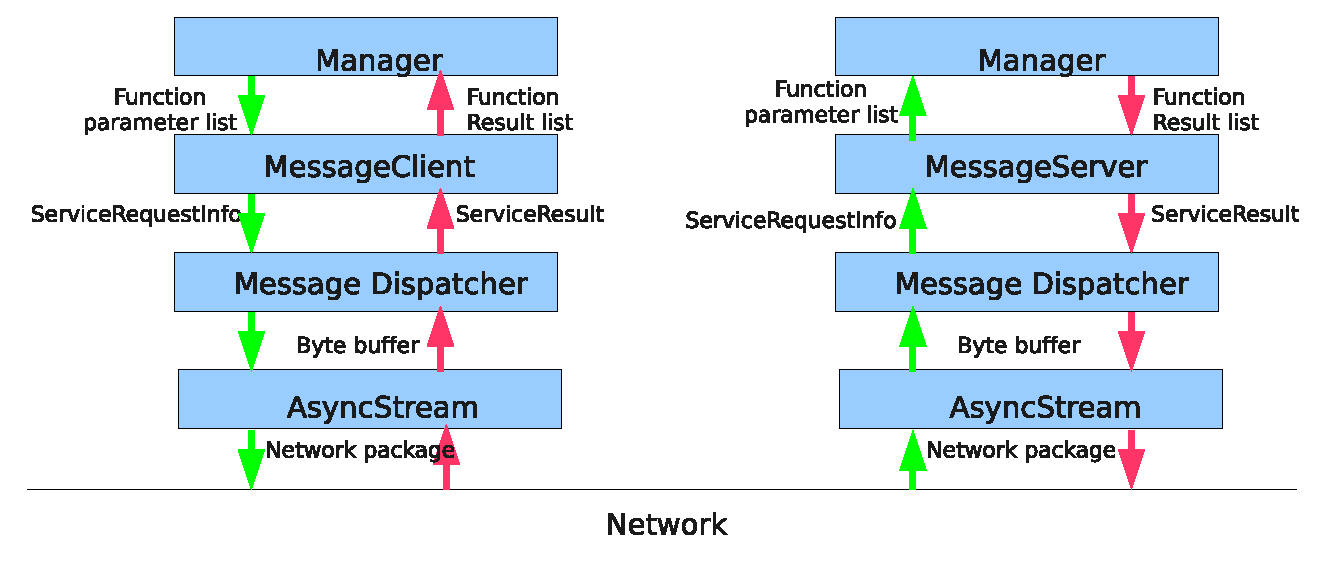
\includegraphics[width=1.0\textwidth]{mf-full.eps}
  \caption{Hierarchical structure of MF-full}\label{fig:mf-full}
\end{figure}

\begin{itemize}
\item The toppest layer, managers, pass service name as well as a list of function parameters to under layer directly, and get back a list of funtion results from under layer.
\item The second layer, MF components, such as MessageServer, MessageClient, and MessageController, will pack funtion parameters into a ServiceRequestInfo object and pass it to under layer.
It also unpack function results from a ServiceResult object which comes from under layer.
Take MessageClient for example, since there maybe more than one managers share one MessageClient instance to request services from other managers, 
MessageClient's major responsiblity is to record which request comes from which manager, then after it receives a reply for certain request, it could deliver the reply to the right caller(manager).
\item The third layer, MessageDispatcher performs serialization/deserialization operations primarily. 
It will serialize ServiceRequestInfo object into byte buffer and then call under layer to write the buffer out, or accept byte buffer from under layer, 
deserialize the buffer into ServiceResult object and then forward the result to upper layer.
\item The bottom layer, AsyncStream, will utilize boost::asio library to write a byte buffer to some peer, or read data from another peer into a byte buffer and then notify the upper layer.
\end{itemize}

\section{Reduce number of messages between managers}

\subsection{Prevent getting permission from Controller}
\index{permission}
In the original design, MessageClient needs to get a permission from MessageController before each time it requests a service.
MessageClient needs to send the service name to MessageController, then MessageController returns back the permission.
The permission contains: a request ID generated by MessageController which is unique in the whole system, the IP and port of the MessageServer which provides requested service.

Obviously, this approach is not efficient enough, because finishing a single request needs to send two messages out,
one to MessageController and the other to MessageServer, so an obvious improvement method is to avoid sending message to MessageController,
that is to say, MessageClient will send the request directly to MessageServer without ask MessageController for permission, see Figure \ref{fig:op_1}.

\begin{figure}[!ht]\centering
  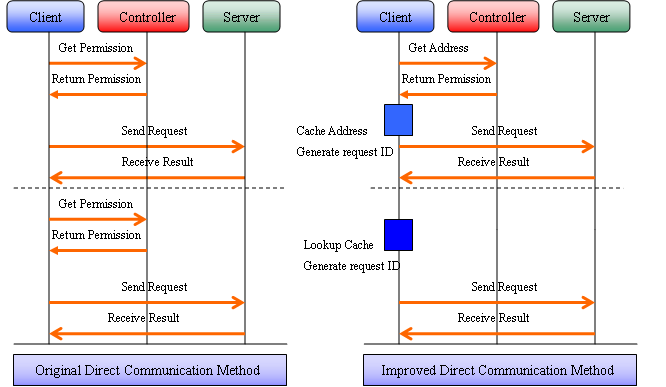
\includegraphics[width=0.65\textwidth]{op_1.png}
  \caption{Improved direct communication method}\label{fig:op_1}
\end{figure}

\index{request ID}
Firstly, the unique request ID doesn't have to be generated by MessageController, it can be generated on MessageClient side also.
Here is my approach, each client gets a 8-bits unique Client ID from MessageController at the boot time, besides each client holds a 24-bits sequential number.
A request ID is generated by concatenating the 8-bits Client ID and 24-bits sequential number into one 32-bits number, then increase the sequential number by one, as shown in Figure \ref{fig:request_ID}.
This ID is unique in the whole system in a long time because
1. different client cannot generate the same request ID because the Client ID parts are different;
2. A client always generate different request ID because the sequential number keeps increasing.

\begin{figure}[!ht]\centering
  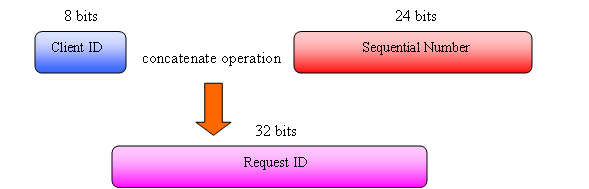
\includegraphics[width=.55 \textwidth]{ID_1.png}
  \caption{Generating the request ID on MessageClient side}\label{fig:request_ID}
\end{figure}

Secondly, MessageServer's address returned by MessageController can be cached on MessageClient, the cache is actually a map looks like $<service's name, server's address>$.
MessageClient needs to get the information from MessageController only the first time it requires the service.

So, in this way, MessageClient need not send message to MessageController to get the permission in most situations.
The number of messages transferred in the whole system is cut down by half, and CPU time is cut down by nearly 30\%.

\subsection{Add a batch request interface}
\index{batch request in MF layer}
There are too many messages transferred in the system, for example, when search a high frequency word, there may be thousands of results found,
then thousands of messages would be transferred. Too many messages cause expensive cost on network traffic, IO wait, synchronization and so on.
So a batch-request interface is introduced to solve this problem. With batch-request interface, library user can send numerous requests out and get their replies by a single call quite efficiently.

Using batch-request interface is much more efficient than sending and then receiving every request individually.
Firstly, in the original design, requests are sent and received one by one, that is to say, after send request 1, client waits until reply 1 arrives, then client begins to send request 2,
if 100 requests are to be sent, the client would enter IO wait status for 100 times.
But When use batch-request interface, as shown in Figure \ref{fig:op_2} , 100 requests can be sent out all together, the client need to enter IO wait status only once waiting until all replies have arrived,
IO wait time can be saved a lot.

\begin{figure}[!ht]\centering
  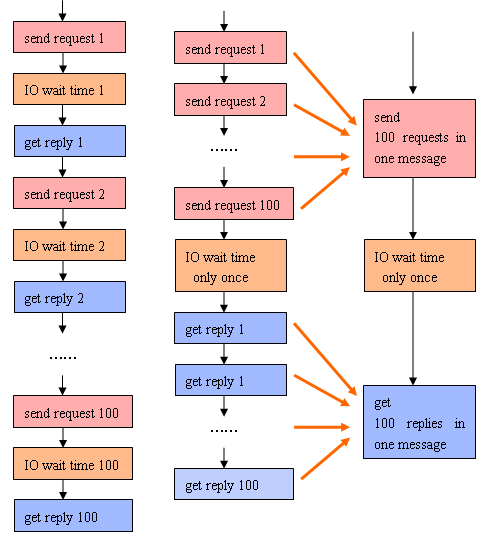
\includegraphics[width=.50\textwidth]{op_2.png}
  \caption{Batch-request saves IO wait time and number of messages}\label{fig:op_2}
\end{figure}

Secondly, using batch-request interface, the number of messages transferred via network is largely reduced, it would save time spending on sending and receiving messages, and synchronization cost.
Since there are multiple threads running on both server and client side waiting for receiving and processing messages,
they must rely on inner-process communication means such as mutex and semaphore to operate on shared internal data structure like linked list, tables and maps,
less messages between client and server side will reduce the number of operations on shared data.

A general batch-request interface is implemented in MessageClientFull class, the interface looks like this:

\begin{lstlisting}[language=C]
class MessageClientFull
{
   /**
    * @brief This function passes a list of requests to the same manager on to
    * MessageClientFull. The MessageClientFull will sends the request to either
    * MessageController or MessageServerFull.
    * @param
    * servicePermissionInfo - it contains information of service name and the server
    * @param
    * serviceRequestInfos - a set of information about request services, each contains
    * the service name and its parameter values.
    * @return
    * true - if the receiver successfully receives these requests
    */
    bool putServiceRequest(const ServicePermissionInfo& servicePermissionInfo,
                         std::vector<ServiceRequestInfoPtr>& serviceRequestInfos);

   /**
    * @brief This function gets a list of results of requested service.
    * The service is requested through function putServiceRequest(..).
    * When the result is not ready, it returns false immediately.
    * @param
    * serviceRequestInfos - a set of service request informations
    * @param
    * serviceResults - a set of service results
    * @return
    * true - Result is ready.
    * @return
    * false - result is not ready.
    */
    bool getResultOfService(const std::vector<ServiceRequestInfoPtr> & serviceRequestInfo,
                        std::vector<ServiceResultPtr> & serviceResults);
}
\end{lstlisting}

Library user passes a vector of requests into MessageClientFull class. Inside MessageClientFull, these requests are split into several sets first, number of requests in each set is less than a user determined value, say, 128.
Then all requests in a set is packed into a single message, there could be multiple messages generated, and these messages are sent to server all together, then the client begin IO wait.
On server side, MessageServerFull class would unpack messages back to vectors of requests, passes them to upper layer, upper layer will process these requests one by one.
When the last request in a message has been processed, MessageServerFull will pack their replies into a single message, send back to client.
The client will wait until all messages return, unpack each message, put all replies into a vector , and return it to caller.
Because everything has been done in MessageClientFull and MessageServerFull, Library User need not modify any code except invoking new batch-request functions instead of original ones, so it's quite easy to use.

Batch-request shrinks total time significantly, it cut down about 60\% time.

\section{Minimize synchronization cost}

\subsection{More efficient implementation of IO wait}
\index{IO wait}
IO wait means in MF, after a client send a request to the server, it must wait for a while until server return the reply.
original MF use busy wait(polling) to implement IO wait, which means, the thread sleeps 1ms each time, when thread wakes up, it checks the status flag to see whether reply arrives, and go on sleeping if not.
With polling, If there are lots of threads active in the system at the same time, threads switching would be very frequently all the time, and receiving a message can not be less than 1ms.

IO wait can be implemented in a more efficient way with a map, a mutex and semaphores.
The map is used to store $<request ID, semaphore>$ pair,
since the map is shared between threads, a mutex should be used to protect the map, semaphores are used to control working threads, make them keep sleeping until reply arrive.

Following pseudo code shows what operations would a working thread do after it sends out the request and before goes to sleep.

\begin{lstlisting}[language=C]
create semaphore
set semaphore=0

lock mutex
Queue[request ID] <- semaphore
unlock mutex

obtain semaphore
\end{lstlisting}

Following code shows what operations would the IO thread do after it receives a reply and wakes corresponding working thread up.

\begin{lstlisting}[language=C]
lock mutex
semaphore <- Queue[request ID]
unlock mutex

release semaphore
\end{lstlisting}

\subsection{Modifications in MF-light}
Class MFControllerLight is rewritten, decrease scope of locks everywhere, and some needless locks are removed.
In original implementation, all managers insert their requests into a global shared rquest queue when they request services, and a thread in MFControllerLight checks the queue from time to time,
gets each request in the queue out and dispatches the request to corresponding managers, the dispatching process is also implemented by sharing a queue between MFControllerLight and each service provider.
The process of receiving reply is similar. After the manager which provides service finish processing the request, it inserts the reply into a global shared reply queue, another thread in MFController checks
the queue from time to time, gets each reply from the queue and dispatches the reply to caller. 

\begin{figure}[!ht]\centering
  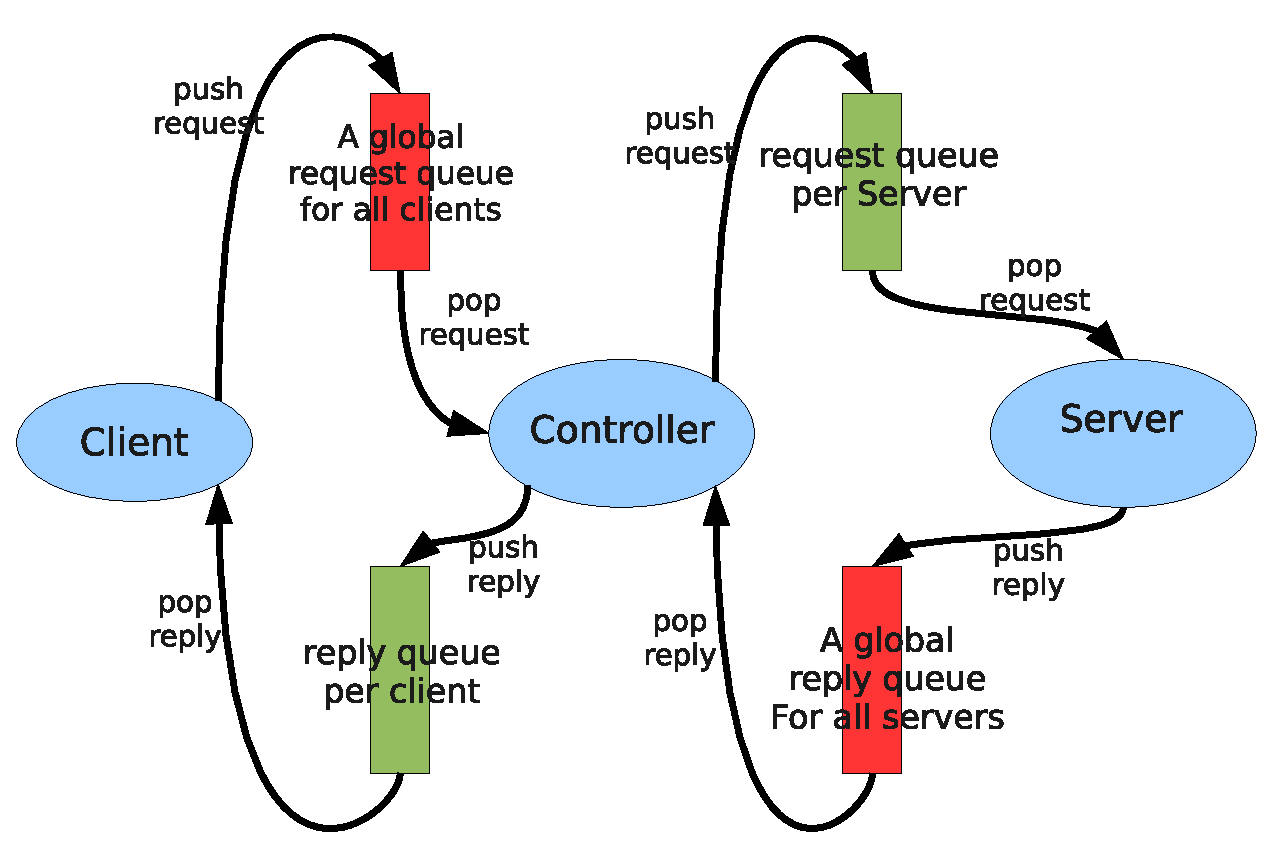
\includegraphics[width=0.7\textwidth]{mf-light-orig.eps}
  \caption{ Queue accesses in original MF-light}\label{fig:mf-light-orig}
\end{figure}

See Figure \ref{fig:mf-light-orig}, queues marked with red color are global queues which are shared between MFControllerLight and all managers in the system,
while queues marked with green color are shared between MFControllerLight and only one manager. This approach is not efficient enough because there are too many
lock operations, access a shared queue need a pair of lock/unlock operation, especially inserting and poping request/reply from a global queue could cause all other managers
paused and waiting to obtain the lock.


A more efficient approch is to let client insert requests into server's request queue directly, similarily, let server insert replies into client's reply queue directly. See Figure \ref{fig:mf-light-now}.
It decreases queue accesses and therefore shrinks lock/unlock operations, so better performance could be achieved.

\begin{figure}[!ht]\centering
  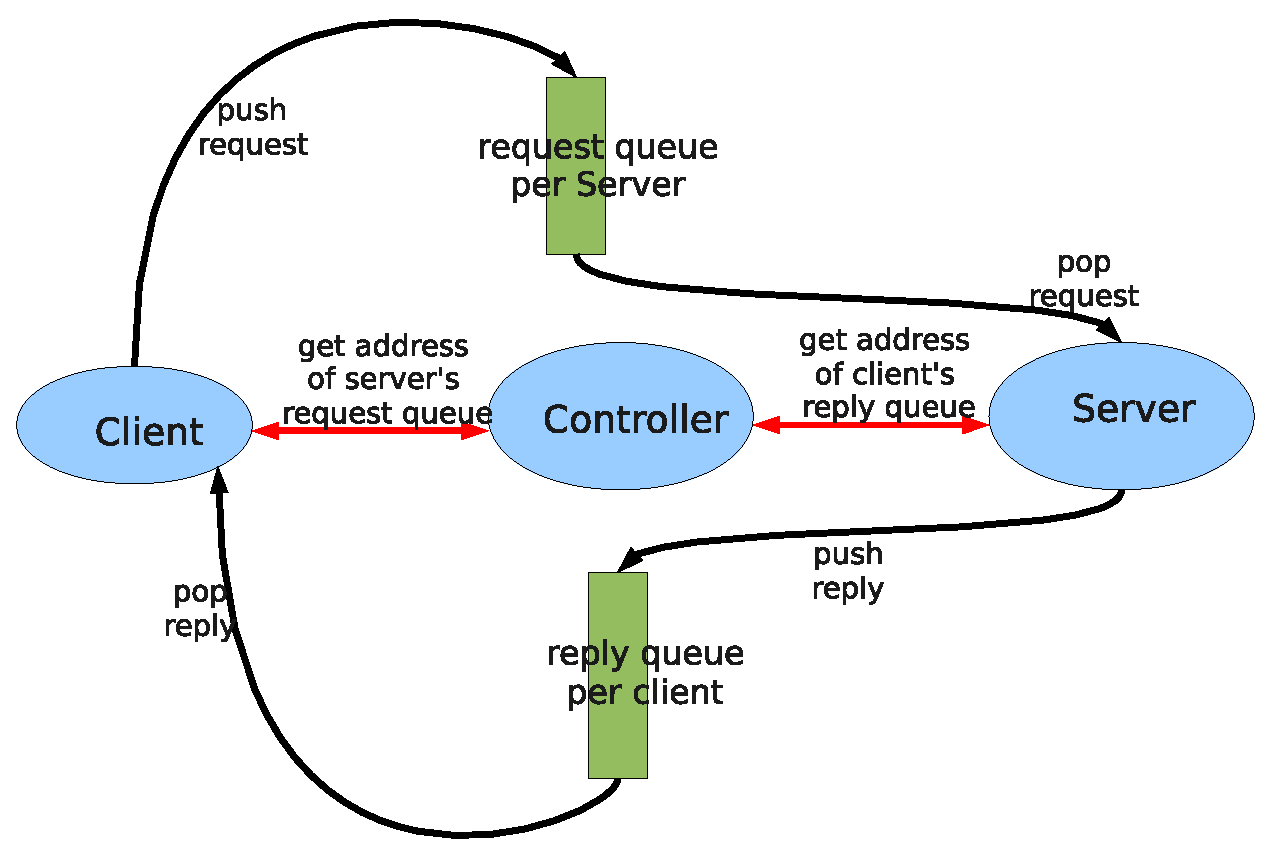
\includegraphics[width=0.7\textwidth]{mf-light-now.eps}
  \caption{ Decrease queue accesses and lock usages in MF-light}\label{fig:mf-light-now}
\end{figure}

Besides, a merge-sort algorithm is written for batch-request when collecting results in client-side, decreasing frequency to invoke a lock shared between server-thread and client-thread.

\section{Use threadpool to accelerate serialization and deserialization}
\index{thread pool}
MF-Full uses asynchronous IO operations to transfer messages between peers, 
which means, there could be multiple working threads sending requests or waiting to receive replies via MF in the upper layer,
but there is only one IO thread working in the underlayer which actually writes packages out and reads packages in.
Another fact is serialization and deserialization operation in MF cost a lot of CPU time, especially boost's serialization.
So a design issue is, which thread should serialization and deserialization operations be executed in?

In original MF, serialization operations are done in working threads, while deserialization operations are done in IO thread, 
as shown in Figure \ref{fig:serial_orig}  . that is to say, the IO thread need to read network packages as well as deserialize them for all working threads. 
There are two disadvantages, the first one is, the throughput decreases because IO thread handle network packages slower than it could have been, 
the second is, all data are deserialized serially, it cannot benifit from more CPU units, if requests are processed fast enough,
then maybe most of working threads would be waiting for IO thread to deserialize packages one by one, in this situation IO thread will be the bottleneck in the whole system.

\begin{figure}[!ht]\centering
  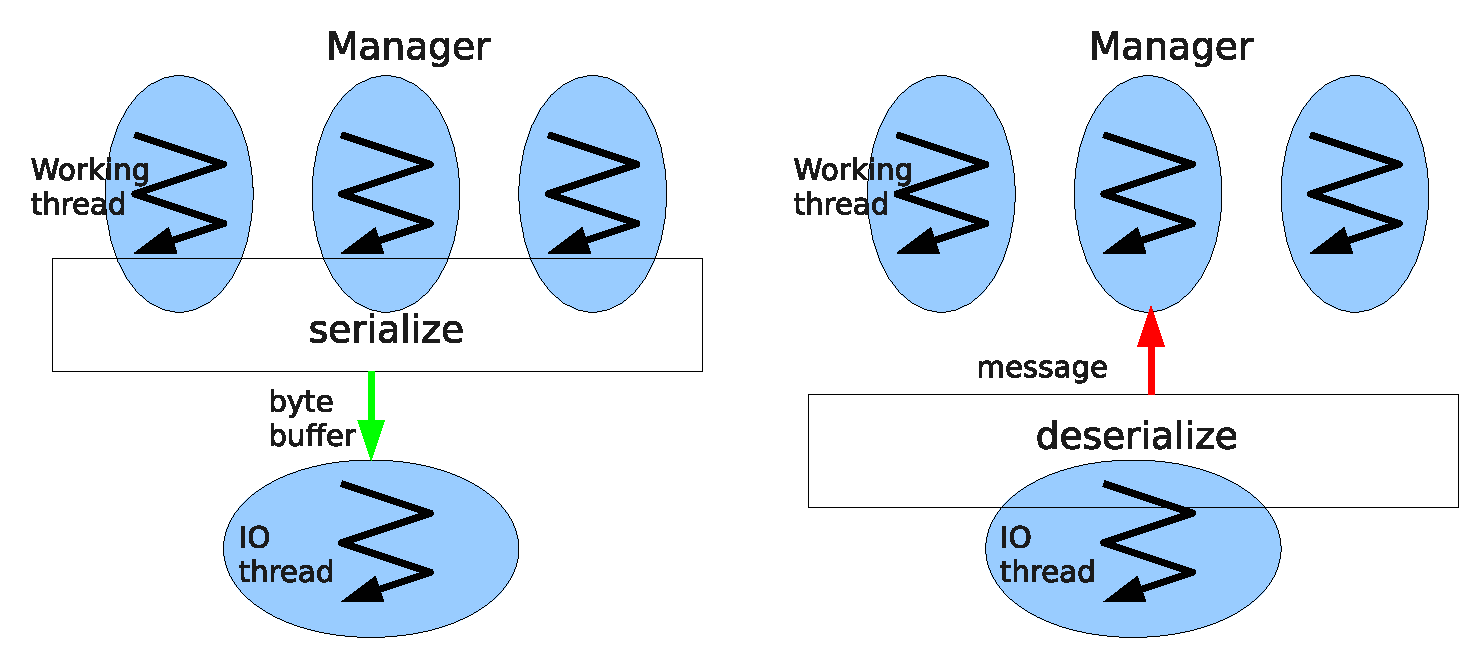
\includegraphics[width=0.7\textwidth]{serial_orig.eps}
  \caption{serialization and deserialization in original MF}\label{fig:serial_orig}
\end{figure}

To accelerate serialization and deserialization operations and make them be processed in parallel,
multiple threads are used to execute the two operations, and a threadpool is written to manage them, see figure  .
There are configurable number of threads in threadpool, working threads will give threadpool the message,
threadpool will find an idle thread and ask the thread to serialize message into byte buffer, the result is sent to IO thread then.
When receive message, IO thread will give threadpool a byte buffer after it accepts a package,
thread pool will find an idle thread and ask the thread to deserialize buffer to message,
then forward the message to corresponding working threads.

\begin{figure}[!ht]\centering
  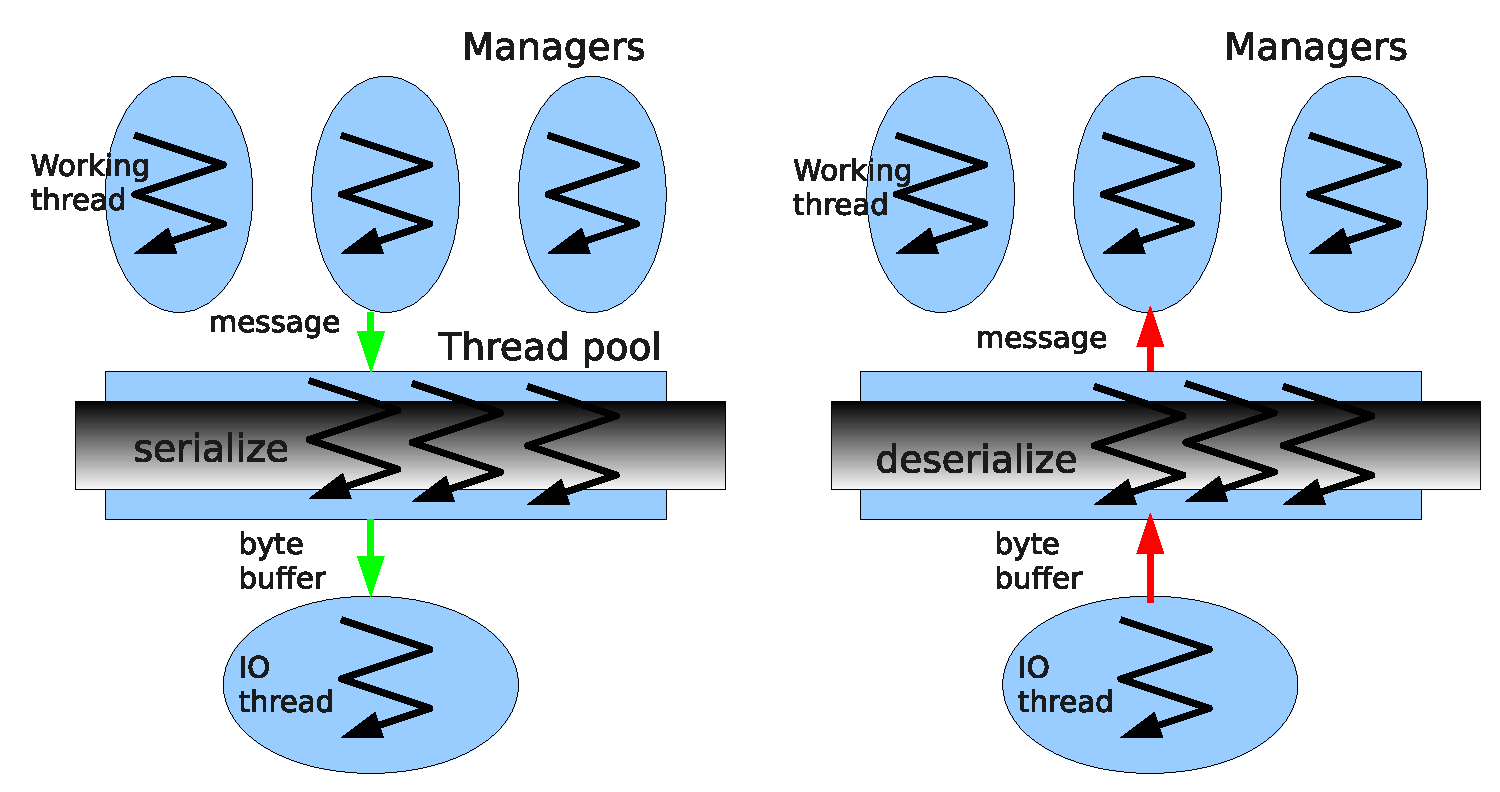
\includegraphics[width=0.7\textwidth]{serial_threadpool.eps}
  \caption{serialization and deserialization using threadpool}\label{fig:serial_theadpool}
\end{figure}


This optimization could utilize multiprocessor system more efficiently,  as well as increase the throughput.

\section{Hierarchical serialization framework}
The data transmitted through MF need to be serialized. Let's firstly
talk about what is serialization.
\subsection{What is serialization? }
\index{serialization}
 In computer science, in the context of data storage and
transmission, serialization
\footnote{http://en.wikipedia.org/wiki/Serialization} is the process
of converting an object into a sequence of bits so that it can be
persisted on a storage medium (such as a file, or a memory buffer)
or transmitted across a network connection link. When the resulting
series of bits is reread according to the serialization format, it
can be used to create a semantically identical clone of the original
object. For many complex objects, such as those that make extensive
use of references, this process is not straightforward.

This process of serializing an object is also called deflating or marshalling an object. The opposite operation, extracting a data structure from a series of bytes, is deserialization (which is also called inflating or unmarshalling).


There are two categories of serialization: human-readable(“text”) and none-human-readable (“binary”).

XML and JSON are the most popular serialization that used for
asynchronous transfer of structured data between client and server
in Ajax web applications.

Mostly binary serialization is more faster than text, we will main
focus on it in MF.
\subsection{Existing serialization libraries }

Boost Serialization, libs11n, Sweet Persist, and Google Protocol
Buffers are libraries that provide support for serialization from
within the C++ language itself. In \textbf{SF1} we mostly use boost
serialization.

\index{Febird}
 Febird\footnote{http://code.google.com/p/febird/} is
a serialization framework that can be used in protocol analysis,
big/small data serialization with high performance. As is said, it
is 30~80 times faster than boost.binary\_archive for some
\textbf{TYPE} and uses less memory. Moreover,it also supports most
STL TYPES and provides high performance.


However,  as we know, for some prime \textbf{TYPE} like int,string
and so on, memory layout copy is the most efficient serialization
(here regardless of endianness.)


Then what is performance difference among those three serialization
methods?

\subsubsection{Serialization comparisons}
We have did some experiments as following:


\begin{itemize}
 \item  serialization of string "izenesoft" 1000,000 times, see
 table \ref{table:1}.

\begin{table} \label{table:1}
\centering
\caption{boost vs Febird vs memory}
\begin{tabular}{|c|c|c|c|} \hline
   & boost & Febird & memory \\  \hline
 elapsed & 3.68 & 0.32  & 0.25 \\  \hline
 length & 12 & 10 & 9 \\
\hline
\end{tabular}
\end{table}


\item  Testing serialization of STL, see table \ref{table:2}.



\begin{table} \label{table:2}
\centering \caption{boost vs Febird vs memory}
\begin{tabular}{|c|c|c|c|} \hline
TYPE  & boost & Febird & memory \\  \hline
 $vector<int>$ & 0.24 & 0.25 & 0.1\\ \hline
 $vector<POD>$ &3.07 & 0.67 & 0.14\\ \hline
 $map<string,int>$ & 5.47 & 1.46  & 1.3\\  \hline
 $map<int, int>$ & 11.75 &7.74  & 7.49\\  \hline
\end{tabular}
\end{table}

where POD refers to
\begin{lstlisting}
struct { int a; int b; int c; int d; }
\end{lstlisting}

\item   Compare cccr\_hash with 3 serialization methods
 (insetion 1000,000 items, key/value : int/string), see table \ref{table:3}


\begin{table}
\centering \caption{boost vs Febird vs memory}  \label{table:3}
\begin{tabular}{|c|c|c|c|} \hline
  & boost & Febird & memory \\  \hline
elapsed & 2.3 & 0.83  & 0.62\\  \hline
\end{tabular}
\end{table}

\end{itemize}
From the obove experiments, we can see that, mostly of time
 memcpy \textgreater Febird \textgreater boost

 Although boost serialization is very easy to be used, it is very
 inefficient.

\subsection{4 level hierarchical serialization}
Our goal for serialization in MF is to design a flexible and scable
serialization framework upon different circumstance.
\begin{itemize}
\item  We can choose different serialization methods in different circumstance, including “binary” and “text” serialization.

\item  MF will use the same serialization as SDB.
\end{itemize}

\subsubsection{Interface}
To achieve the goal, we firstly provide a uniform interface for all
serialization methods through template parameter.
\begin{lstlisting}
 template <typename T> class izene_serialization {
public:
    izene_serialization(const T& dat);
    void write_image(char* &ptr, size_t &size);
};

template <typename T> class izene_deserialization {
public:
    izene_deserialization(const char* ptr, const size_t size);
    void read_image(T& dat);
};
\end{lstlisting}

We can use template specialization to make different serialization
policies  for different \textbf{TYPE}.

\subsubsection{Template specialization}
We design is a 4 levels hierarchical serialization framework, see
table \ref{table:4}. For a given \textbf{TYPE}, 4 serialization
method can be declared.

The upper level will have high priority than low level, i.e. if  top
level serialization method is defined, then only top level
serialization will  take effect and low level serialization will be
used. If customized serialization, memcpy and Febird serialization
are not defined, then default boost serialization will be used as
last choices

\begin{table} \label{table:4}
\centering \caption{Hierarchical serialization framework}
\begin{tabular}{|c|} \hline
customized serialization\\ \hline
memcpy \\ \hline
febird \\ \hline
boost  \\ \hline
\end{tabular}
\end{table}

\index{template derived}
 We use \textbf{template derived} technique to implement the 4
level hierarchical serialization. And \textbf{boost::type\_traits}
lib is used.
\begin{lstlisting}

template <typename T> class izene_serialization {
    typedef typename izene_serial_type< T, IsMemcpySerial<T>::yes,
    IsFebirdSerial<T>::yes>::stype
            stype;
};

template <typename T> class izene_deserialization {
    typedef typename izene_serial_type<T, IsMemcpySerial<T>::yes,
    IsFebirdSerial<T>::yes>::dtype
            dtype;
};


template<typename T, bool isMemcpy = false, bool isFeBird = false>
struct izene_serial_type
{
    typedef izene_serialization_boost<T> stype;
    typedef izene_deserialization_boost<T> dtype;
};

template<typename T>
struct izene_serial_type<T, true, false>
{
    typedef izene_serialization_memcpy<T> stype;
    typedef izene_deserialization_memcpy<T> dtype;
};

template<typename T>
struct izene_serial_type<T, true, true>
{
    typedef izene_serialization_memcpy<T> stype;
    typedef izene_deserialization_memcpy<T> dtype;
};

template<typename T>
struct izene_serial_type<T, false, true>
{
    typedef izene_serialization_febird<T> stype;
    typedef izene_deserialization_febird<T> dtype;
};


template <typename T>
struct IsMemcpySerial{
    enum {yes = ..., no= !yes};
};

template <typename T>
struct IsFebirdSerial{
    enum {yes = 0, no= !yes};
};


\end{lstlisting}




\begin{itemize}
\item For, customized serialization

Just declard the following classes:
\begin{lstlisting}
 template <> class izene_serialization<TYPE> {
....
};
template <> class izene_deserialization<TYPE> {
...
};
\end{lstlisting}
\item For customized memcpy serialization,

Basic type like string, int, float default to be \textbf{memcpy}
serialization. So does std::vector \textless int \textgreater ,
std::vector \textless float \textgreater and so on. For detail,
  please refer source \textbf{izene\_type\_traits.h}


For used defined type \textbf{TYPE}, if we want to use memcpy serialization, the following codes
piece must be provided.

\begin{lstlisting}

MAKE_MEMCPY_SERIALIZATION( TYPE )
template<>
inline void write_image_memcpy<TYPE>(const T& dat, char* &str, size_t& size){
...
}
template<>
inline void read_image_memcpy(T& dat, const char* str, const size_t size){
....
}
\end{lstlisting}

For POD type \textbf{TYPE}, a \textbf{MAKE\_MEMCPY\_TYPE macro} is
enough.

\begin{lstlisting}

MAKE_MEMCPY_TYPE( TYPE )

\end{lstlisting}

For std::vector \textless POD \textgreater, std::pair \textless
POD,POD \textgreater,

boost::tuple \textless POD,POD \textgreater and so on,

only a \textbf{MAKE\_MEMCPY\_SERIALIZATION} macro is needed.

\begin{lstlisting}

MAKE_MEMCPY_SERIALIZATION( TYPE )

\end{lstlisting}

\item For Febird serialization, a macro as following is engough,

But the precondition is that, \textbf{TYPE} itself support
\textbf{Febird} serialization the same as \textbf{boost}
serialization.
\begin{lstlisting}
MAKE_FEBIRD_SERIALIZATION( TYPE )
\end{lstlisting}

\item at last using boost serialization.
\end{itemize}


\subsubsection{Hash function using serialization}
With serialization, hashing function for data with any \textbf{TYPE}
can be defined as follows.
\begin{lstlisting}
 template<typename KeyType> inline ub4 sdb_hashing(const KeyType& key) {
    using namespace izenelib::am::util;

    char* ptr = 0;
    size_t ksize;
    izene_serialization<KeyType> izs(key);
    izs.write_image(ptr, ksize);
    uint32_t convkey = 0;
    char* str = ptr;
    for (size_t i = 0; i < ksize; i++)
        convkey = 37*convkey + (uint8_t)*str++;
    return convkey;
}
\end{lstlisting}


\section{Other Optimizations for MF with new serializations}

\subsection{No VariantType any more}
Old MF use VariantType and boost::any to wrap all kinds of data that
transmitted through MF, and any \textbf{TYPE} has to be registered
first within VariantType with a ID. It is not efficient and
inflexible.


Since any DataType must be serialized to byte streams through MF, we
can use \textbf{MFBuffer} array to represent a given type. Therefore
the data need to be transmitted through MF can be represent
represented as \textbf{MFBufferPtr verctor} in
\textbf{ServiceMessage}, where MFBuffer, MFBufferPtr, and
ServiceMessage are declared as the following: \index{MFBuffer}
\index{ServiceMessage}
\begin{lstlisting}
class MFBuffer
{
public:
    char* data;
    size_t size;
};
 typedef boost::shared_ptr<MFBuffer> MFBufferPtr;

class ServiceMessage {
       MessageHeader mh;
       std::vector<MFBufferPtr> bufferPtrVec;
};

\end{lstlisting}


Two function are provided for encode and decode data into ServiceMessage.
\begin{lstlisting}
template<typename TYPE> inline void mf_serialize(const TYPE& dat,
        ServiceMessagePtr& sm, int idx=0);

template<typename TYPE> inline void mf_deserialize(TYPE& dat,
        const ServiceMessagePtr& sm, int idx=0);

\end{lstlisting}


No VariantType can also save compile time.


\subsection{Both ServiceRequestInfo and ServiceResult are of ServiceMessage Now, conversion cost among them are saved.}
In the old MF, \textbf{ServiceRequestInfo} and
\textbf{ServiceResult} object will be transformed into
\textbf{ServiceMessage} object when dispatched through MF. After
Server or client receive \textbf{ServiceMessage} object, it will
transform it back to \textbf{ServiceRequestInfo} and
\textbf{ServiceResult} object.

\index{ServiceRequestInfo} \index{ServiceResult}
 Since Server and Client know  whether a
received ServiceMessage is ServiceRequest or ServiceResult and their
definition are almost the same. So if both ServiceRequestInfo and
ServiceResult are a ServiceMessage, the cost on conversion among
them  will be saved.
\begin{lstlisting}
typedef ServiceMessage ServiceRequestInfo;
typedef ServiceMessage ServiceResult;
\end{lstlisting}


\subsection{batch request are improved and more flexible}
\index{batch request in application layer} In Wei's design, for batch request,
serveral ServiceRequestInfo are wrapped into a batched ServiceRequestInfo as
a whole. An application level batch request is introduced so that we only need
to bring the data buffers in ServiceRequestInfo to the batch ServiceRequestInfo.
Therefore the transmitted data size for batch request will be reduced much.

With this feature, batch request at application level is available and more flexible.
We just only need to wrap up the data buffers for a batched request at application level.

\subsubsection{batch request at Server Side}
With  the serviceName, server know how to deserialize the buffers in
received \textbf{ServiceRequestInfo}, process the request, and at
last serialize the result into the buffer of ServiceResult.


Moreover, we can view any request as a batch request, and
the only difference for a single request is that, their
batch-process number is only 1, which simplifies the
batch-processing at server side.

\subsubsection{Comparison of two types of batch request implementation}
The Comparison of the two batch request implementation are following:
\begin{itemize}
 \item Batch request at MF level only has fixed batch-processing number(for example 128).  While at application level,
client can determine the batch processing number freely, the only constraint is that,
the serialized data sized can't exceed $2^24$ bytes. So batch request at application layer is much flexible for advanced user.
 \item when there are many requests to send, batch-request at application level still has to
process the requests sequentially at unit of fixed data buffer size, while batch request at MF level can process them in a parallel,
some IO wait time could be saved.
\end{itemize}


\subsection{Macros are provided for better usage}

To make use MF more easy, macros for client request and service
handle are provided. The following are two examples.

Note that we make server side always support batch-request.
\index{MF macro}
\begin{lstlisting}
//for one input parameter and one result: get**(param, result)
#define CLIENT_REQUEST_IMPL_1_1(servicename, MessageClient, param1, result) \
    ServiceRequestInfoPtr req(new ServiceRequestInfo); \
    ServiceResultPtr res; \
    req->setServiceName( servicename ); \
    mf_serialize(param1, req); \
    if ( requestService(servicename, req, res, MessageClient) ) \
    { \
          mf_deserialize(result, res); \
          return true; \
    } \
    return false; \

//for one input parameter and one result: get**(param, result)
#define SERVICE_HANDLE_1_1(request, server, TYPE1, FUNCTION, TYPE2)
\ for(unsigned int i=0; i<request->getBufferNum(); i++){ \
    TYPE1 t1; \
    TYPE2 t2; \
    mf_deserialize(t1, request, i); \
    FUNCTION(t1, t2); \
    mf_serialize(t2, request, i); \
} \
return server.putResultOfService(request); \


\end{lstlisting}

\section{Experiment}

\subsection{Test on message-framework-tesbed}
Compare Wei's optimization with original MF first, then compare Peisheng' optimization over Wei's.

\subsubsection{Experiment setup}
\begin{itemize}
\item 5 process:

 controllerProcess,  LAProcess, IndexProcess, DocumentProcess, Main process

\item MainProcess:  At most 128 requests are sent once via batch-request interface.

\item DocoumentProcess:

parse scd files and pass them  to LAProcess  for LA analysis
then pass the result to IndexProcess for indexing.

\item MainProcess:

It processes  queries.

\end{itemize}


\subsubsection{Experiment result}

\paragraph{Wei's optimization}

\begin{itemize}

\item For MF-light, 65.6\% time is cut down for building index, 56.1\% to 76.8\% time is cut down for querying, the accurate ratio is dependent on query word.

\item For MF-full, 82.9\% time is cut down for building index, 82.5\% to 91\% time is cut down for querying, the accurate ratio is dependent on query word.

\end{itemize}

\paragraph{Peisheng's optimization}

\begin{itemize}

\item  New MF is about twice faster for indexing.

\item  The traffic in MF has been reduced greatly.

The serialized dat size sent through New MF  is only about 10. 4\%
of old MF.  (308150 bytes vs 2908217 bytes.

For this benefits, we can increase batch processing number.

\item  For queries, new MF is about  20\% faster.

MF time (sending and receiving) has been  reduced more than 20\%.


\item  New MF with Memcpy or Febird serialization  is much faster than new MF with boost serialization.

   When we use Febird serialization for ForwardIndex and Document,  the queries time is reduce about 15\%.

\item  Batch Process is much faster than nont batch process number. And batch process at application level is faster than
MF level.

\end{itemize}

\subsection{Test in SF1}

In SF1, we have tried to use currently MF as efficient as possible.

\begin{itemize}

\item Try to use memcpy or Febird serialization for hot data type.
While for Config \textbf{TYPEs}, they are not transmitted frequent
in MF. And we just left it to boost serialization in MF.

\item  Try to add cache for Client requester.

    For example,
    At MainProcee, when a query arrives,
    getCollectionIdByCollectName() to IDManager at DocumentProcee will be firstly called.
    If should be cached, for most of time, CollectionId for a given collectionName is not changed.

\item  Try to use batch process.

\end{itemize}

After use new MF in sf1, the query time has been saved about by 66\%.

\section{Conclusion}
After Wei's and Peisheng's optimization, both the number of messages transferred between managers and the serialization cost are decreased.
Besides, the synchronization cost within multiple threads are cut down, and a thread pool is used for performing serialzation and deserialization operations.
Two types of batch request interface are provided, one is implemented inside MF with a simple and plain interface which is easy to use,
the other is at application layer and Peisheng provides some macros to help programming, which is situable for advanced user.
We recomment to use batch request interface as much as possible.

\printindex
%--------------------------------------------------
\end{document}
